\chapter{IPython Notebook}
\label{ch:notebook}

\section{Getting Started}

IPython Notebook is an interactive web-based tool which combines code execution, mathematics, and rich media output.

You can find a plethora of information at \href{http://ipython.org/ipython-doc/dev/notebook/index.html}

Let's get started.

To open a notebook window, open a terminal and initiate Ureka:

\begin{alltt}
\termtab ur_setup common ssbx
\termtab ipython notebook
\end{alltt}

Opening the notebook this way will create a new tab in your browser. All subsequent interactions will now
be through the browser and the terminal will be running the server that the browser interacts with.

IPython Notebook will look for notebook files (.ipynb) in the directory where you started the notebook in.


\section{Plotting Inline}

A unique feature that the notebook has is the ability to plot inline.

You can initiate inline plotting two ways.

From the terminal:

\begin{alltt}
\termtab ur_setup common ssbx
\termtab ipython notebook --pylab inline
\end{alltt}

From the notebook window:

\begin{alltt}
\pytab \%pylab inline
\end{alltt}

Without telling the notebook to plot inline, plots will pop up in a separate window just as they normally
would plotting in the python terminal.

\section{Notebook Examples}


%%%%%%%%%%%%%%%%
\begin{figure}[tbp]
  \centering
    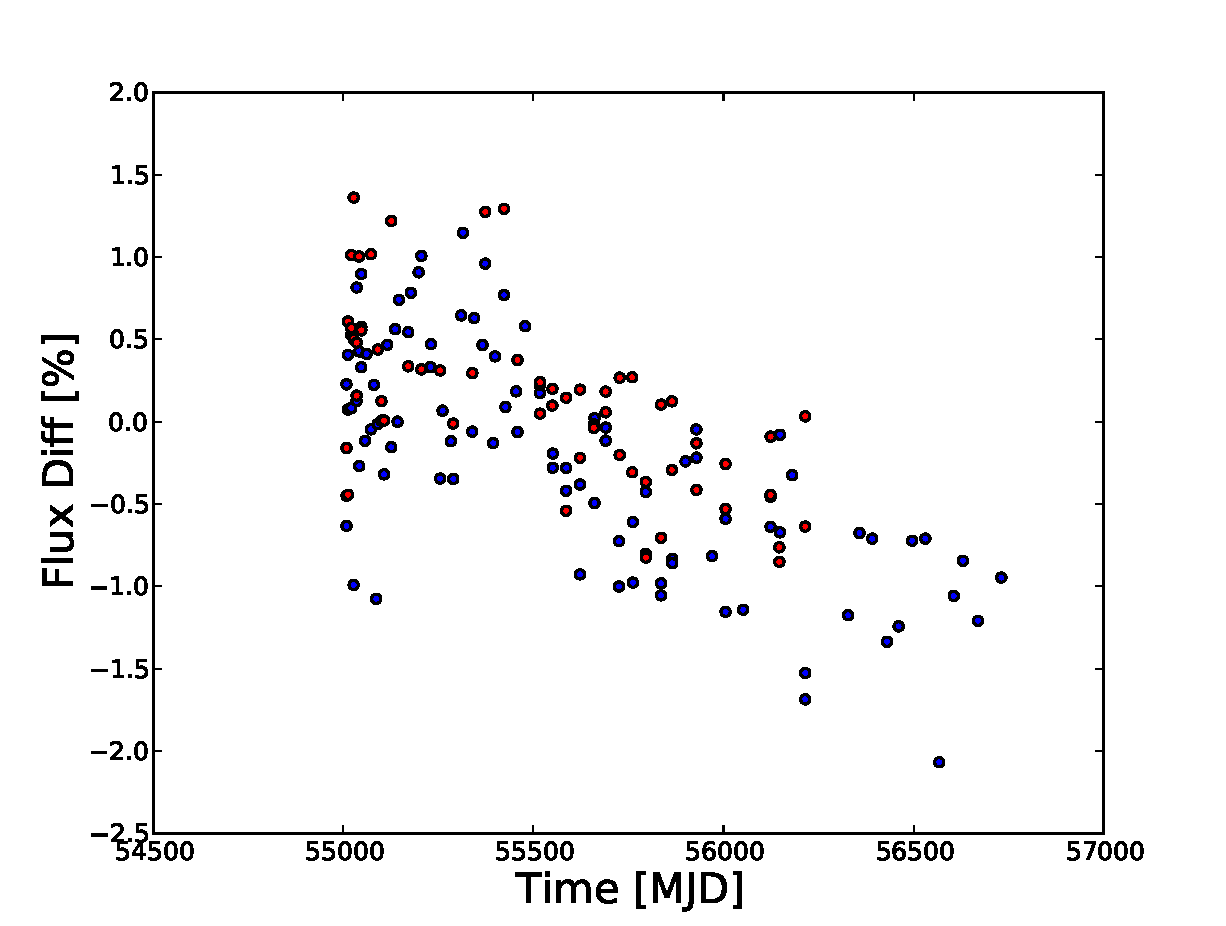
\includegraphics[scale=0.55]{flux_vs_time_1.pdf}
    \caption{Our first plot.}
  \label{fig:splot}
\end{figure}
%%%%%%%%%%%%%%%%


